
\documentclass[a4paper,12pt,oneside]{scrbook}

%----------------------------------------------------------------------------------------
% PAQUETES Y ESTILO
%----------------------------------------------------------------------------------------

% IMPORTANTE
% Para poner barrabaja en una url hay que cambiar '_' por '\textunderscore'

%========================================================================================
% PAQUETES
%========================================================================================

\usepackage[spanish]{babel} % Indicar idioma español
\usepackage[utf8]{inputenc} % Poder poner tildes directamente
\usepackage{graphicx} % Para incluir gráficos
\usepackage{cite} % Para crear referencias
\usepackage{svg} % Para usar imágenes en formato vectorial
\usepackage{float} % Para modificar como aparecen las imagenes
\usepackage{listings} % Para introducir código
\usepackage{times}
\usepackage{color} % para añadir colores
\usepackage{hyperref}  % Para que se creen enlaces en el documento (a otras partes o a la web)
\usepackage{AnonymousPro}
\usepackage{url}
\usepackage[Bjornstrup]{fncychap} % Para poner los títulos de los capítulos más bonitos
\usepackage{fancyhdr} % Para configurar las cabeceras y los piés de página
\usepackage{titling} % Para usar la información del documento en otras partes de él
\usepackage{caption}
\usepackage{minted}

%========================================================================================
% ESTILO
%========================================================================================

%----------------------------------------------------------------------------------------
% RUTAS PARA LAS IMAGENES
%----------------------------------------------------------------------------------------

\graphicspath{{./figuras/}}

%----------------------------------------------------------------------------------------
% ARREGLO PARA EL INDICE DE FIGURAS
%----------------------------------------------------------------------------------------

\makeatletter
\renewcommand*\l@figure{\@dottedtocline{1}{1em}{3.2em}}
\makeatother

%----------------------------------------------------------------------------------------
% TIPOGRAFIA
%----------------------------------------------------------------------------------------

\renewcommand{\familydefault}{\sfdefault} % Cambia la tipografía de todo el documento
\setlength{\parskip}{2mm} % Define la distancia entre parrafos (por defecto = 0)

%----------------------------------------------------------------------------------------
% CABECERAS Y PIES DE PAGINA
%----------------------------------------------------------------------------------------
\pagestyle{fancy}
\fancyhf{}
\fancyhead[CE,CO]{\leftmark}
\fancyhead[LE,RO]{\thepage}
\fancyfoot[RE,LO]{Ander Granado Masid}
\fancyfoot[LE,RO]{\thepage}

\renewcommand{\headrulewidth}{2pt}
\renewcommand{\footrulewidth}{1pt}

%----------------------------------------------------------------------------------------
% ENLACES
%----------------------------------------------------------------------------------------

\hypersetup{
	colorlinks,
	citecolor=black,
	filecolor=black,
	linkcolor=black,
	urlcolor=black
}

%----------------------------------------------------------------------------------------
% NUMERO DE PROFUNDIDAD DE NUMERACION DE CONENIDOS
%----------------------------------------------------------------------------------------
\setcounter{tocdepth}{3}
\setcounter{secnumdepth}{3}

%----------------------------------------------------------------------------------------
% CODIGO
%----------------------------------------------------------------------------------------

% Parte para los comandos (con lstlisting)
\definecolor{gray95}{gray}{.95}
\definecolor{gray85}{gray}{.80}
\definecolor{gray45}{gray}{.45}
\definecolor{myturquoise}{RGB}{0, 128, 128}
\definecolor{mypink}{RGB}{177,48,112}
\definecolor{myblue}{RGB}{56,133,231}

\lstset{ 
	frame=Ltb,
	framerule=0pt,
	aboveskip=0.5cm,
	framextopmargin=3pt,
	framexbottommargin=3pt,
	framexleftmargin=0.2cm,
	framesep=0pt,
	rulesep=2.0pt,
	backgroundcolor=\color{gray95},
	rulesepcolor=\color{black},
	%
	stringstyle=\ttfamily,
	showstringspaces = false,
	basicstyle=\small\ttfamily,
	commentstyle=\color{gray45},
	keywordstyle=\bfseries,
	%
	numbers=left,
	numbersep=15pt,
	numberstyle=\tiny,
	numberfirstline = false,
	breaklines=true,
}

% Minimizar fragmentado de listados
%\lstnewenvironment{listing}[1][]
%{\lstset{#1}\pagebreak[0]}{\pagebreak[0]}

% Estilo de codigo para la consola
\lstdefinelanguage{none}{}
\lstdefinestyle{consola}{
	language=none,
	breaklines=true,
	basicstyle=\footnotesize\bf\ttfamily,
	backgroundcolor=\color{gray85},
	rulesepcolor=\color{myturquoise},
	numbers=none,
}

% Parte para el código (con minted) (minted es mejor para código que lstlisting)
\usemintedstyle{borland}

%----------------------------------------------------------------------------------------
% INFORMACION DEL DOCUMENTO
%----------------------------------------------------------------------------------------

\title{Virtualización ligera para sistemas embebidos con aplicaciones robóticas usando ROS y Docker}
\author{Ander Granado Masid}
\date{\today}

%========================================================================================
% DOCUMENTO
%----------------------------------------------------------------------------------------
\begin{document}

\frontmatter % Define la parte inicial del libro, que suele ir compuesto por:

\begin{titlepage}
	
\includegraphics[width=0.3\textwidth]{portada/logoEHU}
	\hspace{\fill}
	
\includegraphics[width=0.3\textwidth]{portada/logoEUI}
	\vspace{1.5cm}
	\begin{center}
		
		\LARGE{Administración de Sistemas}
		
		\vskip1.5cm
		
		\Huge{\textbf{\thetitle}}
		
		\vskip1.5cm
		
		
\includegraphics[width=10cm]{portada/docker-ros-logo}
		
		\vskip1.5cm
		
		\Large{\theauthor}
	
		\vskip 1cm
		
		\textit{\today}
	\end{center}
	\vspace{2cm}
	\hspace{\fill}
	
\includegraphics[width=3cm]{portada/cclogolarge}
	\hspace{1cm}
	
\includegraphics[width=2cm]{portada/by-sa}
	\hspace{\fill}
\end{titlepage} % Título personalizado
\tableofcontents % Indice de contenidos
\listoffigures % Indice de figuras

%----------------------------------------------------------------------------------------

\mainmatter % Define la parte frincipal del libro, el contenido
\part{Introducción}
	\chapter{Objetivo}
En el siguiente documento tiene como objetivo desarrollar un sistema virtualizado para controlar un vehículo robótico. Este sistema dispondrá de diferentes módulos que estarán conectados entre sí e interactuarán entre ellos. Para desarrollarlo se hará uso de ROS y Docker. El sistema estará pensado para funcionar dentro de una Raspberry Pi. En el siguiente capítulo se explicará en profundidad todas las herramientas que usaremos para desarrollarlo, tanto de hardware como de software.
	\chapter{Herramientas utilizadas}

\section{Hardware}
Aunque el vehículo dispone de numeroso hardware, en esta sección solo hablaremos sobre el hardware para el cual nosotros vamos a programar. En este caso todo nuestro sistema se montará en una Raspberry pi, aunque el desarrollo del sistema lo haremos en los PCs con arquitectura x86.

	\subsection{Raspberry Pi}
	Raspberry Pi es un ordenador de placa reducida que debido a us bajo coste (35 \$) y su pequeño tamaño, es ampliamente usado en sistemas de bajo coste, sistemas embebidos o en entornos educativos. Existen dos principales modelos, la Raspberry Pi y la Raspberry Pi 2. La Raspberry Pi a su vez cuenta con 4 diferentes submodelos, el A, el A+, el B y el B+.
	
	Aunque cuenta con diferentes submodelos con diferentes especificaciones, las características generales de la Raspberry Pi son \cite{rpi-wikipedia}:
	
	\begin{itemize}
		\item SoC (System on Chip) Broadcom BCM2835:
			\begin{itemize}
				\item CPU ARM 1176JZF-S a 700 MHz single-core (familia ARM11)
				\item GPU Broadcom VideoCore IV (OpenGL ES 2.0, MPEG-2 y VC-1, 1080p30 H.264/MPEG-4 AVC3)
			\end{itemize}
		\item Memoria SDRAM: 256 MB (en el modelo A) o 512 MB (en el modelo B), compartidos con la GPU
		\item Puertos USB 2.0: 1 (en el modelo A), 2 (en el modelo B) o 4 (en el modelo B+)
		\item 10/100 Ethernet RJ-45 (en el Modelo B)
		\item Salidas de video:
			\begin{itemize}
				\item Conector RCA (PAL y NTSC)
				\item HDMI (rev1.3 y 1.4)
				\item Interfaz DSI para panel LCD
			\end{itemize}
		\item Salidas de audio:
			\begin{itemize}
				\item Conector de 3.5 mm
				\item HDMI
			\end{itemize}
		\item Puertos GPIO: 8 o 17 (en el caso de las versiones +)
	\end{itemize}
	
	El segundo modelo de Raspberry Pi, conocido como Paspberry Pi 2, añade mejoras notables con respecto a la anterior generación. Sus características básicas son:
	
	\begin{itemize}
		\item SoC Broadcom BCM2836:
			\begin{itemize}
				\item 900 MHz quad-core ARM Cortex A7
				\item GPU Broadcom VideoCore IV (OpenGL ES 2.0, MPEG-2 y VC-1, 1080p30 H.264/MPEG-4 AVC3)
			\end{itemize}
		\item 1GB memoria SDRAM, compartida con la GPU
		\item 4 puertos USB 2.0
		\item 10/100 Ethernet RJ-45
		\item Salidas de video:
		\begin{itemize}
			\item Conector RCA (PAL y NTSC)
			\item HDMI (rev1.3 y 1.4)
			\item Interfaz DSI para panel LCD
		\end{itemize}
		\item Salidas de audio:
		\begin{itemize}
			\item Conector de 3.5 mm
			\item HDMI
		\end{itemize}
		\item 17 puertos GPIO
	\end{itemize}
	

\section{Software}
Para lograr dicho objetivo anteriormente descrito, se hace uso de una serie de herramientas, entre las cuales se incluye Docker y ROS.

	\subsection{Docker}
	Docker es una plataforma abierta para aplicaciones distribuidas para desarrolladores y administradores de sistemas\cite{docker-web}. Docker automatiza el despliegue de contenidos de software proporcionando una capa adicional de abstracción y automatización de virtualización a nivel de sistema operativo en Linux \cite{docker-wikipedia}. Docker utiliza características de aislamiento de recursos del kernel de Linux, 
	
		\subsubsection{Funcionamiento de Docker}
		Docker se basa en el el principio de los contenedores. Cada contenedor consta de una serie de aplicaciones y/o librerías que se ejecutan de manera independiente del OS (Sistema Operativo) principal, pero que usan el kernel Linux del sistema operativo anfitrión. Para hacer esto se hacen uso de diferentes técnicas tales como cgroups y espacios de nombres (namespaces) para permitir que estos contenedores independientes se ejecuten dentro de una sola instancia de Linux. De esta manera se logra reducir drásticamente el consumo de recursos de hardware, a cambio de que las librerías, aplicaciones o sistemas operativos deban ser compatibles con linux y ser compatibles con la arquitectura del hardware en la que se están ejecutando (x86, ARM, SPARC,...).
		
		Mediante el uso de contenedores, los recursos pueden ser aislados, los servicios restringidos, y se otorga a los procesos la capacidad de tener una visión casi completamente privada del sistema operativo con su propio identificador de espacio de proceso, la estructura del sistema de archivos, y las interfaces de red. Los contenedores comparten el mismo kernel, pero cada contenedor puede ser restringido a utilizar sólo una cantidad definida de recursos como CPU, memoria y E/S. \cite{docker-wikipedia}.

	\subsection{ROS}
	ROS (Robot Operating System) es un framework flexible para desarrollar software para robots. Es una colección de herramientas, librerías que tratan de simplificar la creación de aplicaciones complejas y robustas para todo tipo de sistemas robóticos \cite{ros-web}.
	
	ROS provee los servicios estándar de un sistema operativo tales como abstracción del hardware, control de dispositivos de bajo nivel, implementación de funcionalidad de uso común, paso de mensajes entre procesos y mantenimiento de paquetes. Está basado en una arquitectura de grafos donde el procesamiento toma lugar en los nodos que pueden recibir, mandar y multiplexar mensajes de sensores, control, estados, planificaciones y actuadores, entre otros \cite{ros-wikipedia}.


	Las áreas que incluye ROS son:
	\begin{itemize}
		\item Un nodo principal de coordinación.
		\item Publicación o subscripción de flujos de datos: imágenes, estéreo, láser, control, actuador, contacto, etc.
		\item Multiplexación de la información.
		\item Creación y destrucción de nodos.
		\item Los nodos están perfectamente distribuidos, permitiendo procesamiento distribuido en múltiples núcleos, multiprocesamiento, GPUs y clústeres.
		Login.
		\item Parámetros de servidor.
		\item Testeo de sistemas.
	\end{itemize}

\part{Docker}
	\chapter{Introducción a Docker}
Tras haber explicado anteriormente a grandes rasgos el funcionamiento de Docker, es conveniente antes de lanzarnos a la creación del sistema saber como crear y configurar los contenedores de Docker que conformarán el sistema. En este capítulo se explicará como empezar a trabajar con Docker, desde instalarlo y como empezar a usarlo hasta como se usan los Dockerfiles para lanzar contenedores personalizados.

	\section{Instalación}
	Lo primero que haremos será instalar Docker en nuestro sistema. En nuestro caso tenemos un sistema Ubuntu instalado en una máquina virtual, ya que nuestro hardware cuenta con SO Windows. Instalar Docker en cualguier distribución basada en Debian es tan sencillo como seguir los siguientes pasos \cite{docker-install}:
	
	\lstset{language=bash, breaklines=true, basicstyle=\footnotesize}
	\begin{enumerate}
		\item Comprobar si tenemos curl instalado
		\begin{lstlisting}[style=consola]
$ which curl
		\end{lstlisting}
		En caso de que no este instalado, instalarlo mediante:
		\begin{lstlisting}[style=consola]
$ sudo apt-get update
$ sudo apt-get install curl
		\end{lstlisting}
		\item Instalar Docker mediante el siguiente comando:
		\begin{lstlisting}[style=consola]
$ curl -sSL https://get.docker.com/ | sh
		\end{lstlisting}
		\item Comprobar que Docker se ha instalado correctamente.
		\begin{lstlisting}[style=consola]
$ docker run hello-world
		\end{lstlisting}
			Si ejecutamos el comando anterior y nos muestra información sobre Docker, ya hemos terminado de instalar Docker.
	\end{enumerate}
	
	\section{Uso básico de Docker}
	Para hacer uso de Docker necesitamos trabajar desde la terminal. La forma básica para trabajar con Docker es la siguiente:
	
	\begin{lstlisting}[style=consola]
$ docker [subcomando de docker] [parametros]
	\end{lstlisting}

	De esa manera primero indicamos que queremos usar Docker y a continuación indicamos que es lo que queremos hacer. En el ejemplo anterior hemos usado \textit{run} para ejecutar un contenedor de Docker. Por último introducimos los diferentes parámetros. La lista completa de comandos que acepta Docker se puede ver de las siguiente manera:
	% basicstyle=\scriptsize
	\begin{lstlisting}[style=consola,numbers=left]
$ docker --help
Usage: docker [OPTIONS] COMMAND [arg...]
docker daemon [ --help | ... ]
docker [ --help | -v | --version ]

A self-sufficient runtime for containers.

Options:

--config=~/.docker              Location of client config files
-D, --debug=false               Enable debug mode
-H, --host=[]                   Daemon socket(s) to connect to
-h, --help=false                Print usage
-l, --log-level=info            Set the logging level
--tls=false                     Use TLS; implied by --tlsverify
--tlscacert=~/.docker/ca.pem    Trust certs signed only by this CA
--tlscert=~/.docker/cert.pem    Path to TLS certificate file
--tlskey=~/.docker/key.pem      Path to TLS key file
--tlsverify=false               Use TLS and verify the remote
-v, --version=false             Print version information and quit

Commands:
attach    Attach to a running container
build     Build an image from a Dockerfile
commit    Create a new image from a container's changes
cp        Copy files/folders from a container to a HOSTDIR or to STDOUT
create    Create a new container
diff      Inspect changes on a container's filesystem
events    Get real time events from the server
exec      Run a command in a running container
export    Export a container's filesystem as a tar archive
history   Show the history of an image
images    List images
import    Import the contents from a tarball to create a filesystem image
info      Display system-wide information
inspect   Return low-level information on a container or image
kill      Kill a running container
load      Load an image from a tar archive or STDIN
login     Register or log in to a Docker registry
logout    Log out from a Docker registry
logs      Fetch the logs of a container
pause     Pause all processes within a container
port      List port mappings or a specific mapping for the CONTAINER
ps        List containers
pull      Pull an image or a repository from a registry
push      Push an image or a repository to a registry
rename    Rename a container
restart   Restart a running container
rm        Remove one or more containers
rmi       Remove one or more images
run       Run a command in a new container
save      Save an image(s) to a tar archive
search    Search the Docker Hub for images
start     Start one or more stopped containers
stats     Display a live stream of container(s) resource usage statistics
stop      Stop a running container
tag       Tag an image into a repository
top       Display the running processes of a container
unpause   Unpause all processes within a container
version   Show the Docker version information
wait      Block until a container stops, then print its exit code

Run 'docker COMMAND --help' for more information on a command.
	\end{lstlisting}
	
	Como se puede observar existen diferentes comandos que nos permitirán configurar Docker, obtener información sobre el y tratar con las imágenes y los contenedores de Docker. A continuación vamos a explicar algunos de ellos para poder empezar a trabajar con Docker. 
	
	\subsection{\textit{run}}
	El comando esencial para empezar a trabajar con Docker es el comando \textbf{\emph{run}}. Para poder lanzar directamente un contenedor de Docker, se usa el comando \textit{run}.
	
	\begin{lstlisting}[style=consola]
$ docker run ubuntu:trusty
	\end{lstlisting}
	
	Con el comando anterior hemos lanzado un contenedor de Docker que lleva Ubuntu. Lo primero que hace Docker para lanzar una imagen es comprobar si ya tiene en local la imagen desde la que se va a crear el contenedor. En caso de no tenerla accederá a unos repositorios llamados Docker Hub, donde se encuentran una gran cantidad de \textbf{\emph{Dockerfiles}}. Los \emph{Dockerfiles} son los archivos que sirven para generar esas imágenes (veremos más adelante como funcionan estos archivos especiales). Una vez Docker genere la imagen a partir del \textit{Dockerfile} ejecutará el contenedor, que a grandes rasgos es una instancia de la imagen.
	
	\subsection{\textit{ps}}
	Podremos observar los contenedores Docker que tenemos lanzados mediante el comando \textbf{\emph{ps}} de Docker.
	
	\begin{lstlisting}[style=consola,numbers=left]
$ docker ps
CONTAINER ID        IMAGE               COMMAND                  CREATED             STATUS              PORTS               NAMES
	\end{lstlisting}
	
	Aunque hemos lanzado un contenedor, mediante el comando \emph{ps} de Docker vemos que en realidad no hay ningún contenedor en ejecución. Si no le indicamos ningún parámetro al comando \emph{ps}, solo nos mostrará los contendores en ejecución. Para mostrar todos, se hace uso hay que indicarselo con \emph{-a}.
	
	Si nosotros hemos lanzado un contenedor, ¿Porqué no se está ejecutando? Esto es porque los contenedores de Docker solo se mantienen en ejecución mientras el comando con el que se han iniciado este activo \cite{docker-run}.
	
	Para poder probar el comportamiento por defecto del comando \emph{ps}, vamos a crear un contenedor demonizado, un contenedor que se ejecutará indefinidamente hasta que lo paremos. Esto es muy habitual en Docker, ya que las aplicaciones hechas con Docker suelen diseñarse para funcionar 24/7, como por ejemplo servidores web. Lo haremos de la siguiente manera.
	
	\begin{lstlisting}[style=consola]
$ docker run -d ubuntu:14.04 /bin/sh -c "while true; do echo hello world; sleep 1; done"
	\end{lstlisting}
	
	Con el \textbf{-d} lo que logramos es que se siga ejecutando el contenedor en segundo plano, como si fuera un demonio (daemon), un proceso que esta siempre en ejecución. También debemos darle algo para hacer, ya que si no, tal y como hemos comentado antes, finalizará la ejecución. Esto lo logramos mediante un bucle infinito en shell script, que es lo que pasamos como parámetro entre comillas. Si ahora ejecutamos el comando \emph{ps}, comprobaremos que tenemos una máquina en ejecución.
	
	\begin{lstlisting}[style=consola,numbers=left]
$ docker ps
CONTAINER ID        IMAGE               COMMAND                  CREATED             STATUS              PORTS               NAMES
40f5c913912e        ubuntu              "/bin/sh -c 'while tr"   2 seconds ago       Up 2 seconds                            adoring_euclid
	\end{lstlisting}
	
	\subsection{\textit{inspect}}
	En caso de que queramos obtener más información sobre un contenedor de Docker, podemos usar el comando \textbf{\emph{inspect}} de Docker. La forma más básica de trabajar con este comando es la de utilizar como parámetro el ID o nombre de la maquina. Este comando nos devolverá por la salida estándar un JSON con una gran cantidad de parámetros que nos indican diferentes aspectos sobre el contenedor. También se pueden obtener solo un parámetro o un grupo de parámetros en concreto. En el siguiente ejemplo se muestra su uso, para obtener toda la información y para obtener un dato, en este caso la dirección IP del contenedor.
	
	\begin{lstlisting}[style=consola,numbers=left]
$ docker inspect adoring_euclid
# ...
# ... Se omite la salida por ser demasiado grande
# ...
$ docker inspect --format='{{.NetworkSettings.IPAddress}}' adoring_euclid
172.17.0.3
	\end{lstlisting}

	\subsection{\textit{stop} y \textit{kill}}
	En caso de que queramos matar un contenedor, podremos hacerlo mediante el comando \textbf{\emph{stop}} o mediante el comando \textbf{\emph{kill}} de Docker. El primero mata directamente el contenedor, de manera análoga al kill de linux, a diferencia del otro, que detiene la ejecución de una manera más segura.
	
	\begin{lstlisting}[style=consola,numbers=left]
$ docker ps
CONTAINER ID        IMAGE               COMMAND                  CREATED             STATUS              PORTS               NAMES
40f5c913912e        ubuntu              "/bin/sh -c 'while tr"   2 seconds ago       Up 2 seconds                            adoring_euclid
$ docker stop 40f5c913912e
40f5c913912e
$ docker ps
CONTAINER ID        IMAGE               COMMAND                  CREATED             STATUS              PORTS               NAMES

	\end{lstlisting}
	
	\subsection{\textit{rm}}
	Hay que tener en cuenta que ni stop ni kill eliminan el contenedor, sino que detienen su ejecución. El contenedor, junto con toda la información que tiene, sigue almacenado. Si queremos eliminar un contenedor definitivamente lo que debemos hacer es usar el comando \textbf{\emph{rm}} de Docker.
	
	\begin{lstlisting}[style=consola,numbers=left]
$ docker ps
CONTAINER ID        IMAGE               COMMAND             CREATED             STATUS              PORTS               NAMES
$ docker run -d ubuntu:14.04 /bin/sh -c "while true; do echo hello world; sleep 1; done"
5abaece69cbd445e69cae61cef6de9f42e2561eacb4b8969024c922eec348a5d
$ docker ps
CONTAINER ID        IMAGE               COMMAND                  CREATED             STATUS              PORTS               NAMES
5abaece69cbd        ubuntu:14.04        "/bin/sh -c 'while tr"   3 seconds ago       Up 2 seconds                            mad_ardinghelli
$ docker stop mad_ardinghelli
mad_ardinghelli
$ docker ps
CONTAINER ID        IMAGE               COMMAND             CREATED             STATUS              PORTS               NAMES
$ docker ps -a
CONTAINER ID        IMAGE               COMMAND                  CREATED             STATUS                       PORTS               NAMES
5abaece69cbd        ubuntu:14.04        "/bin/sh -c 'while tr"   5 minutes ago       Exited (137) 4 minutes ago                       mad_ardinghelli
$ docker rm mad_ardinghelli
mad_ardinghelli
$ docker ps -a
CONTAINER ID        IMAGE               COMMAND                  CREATED             STATUS                       PORTS               NAMES
	\end{lstlisting}	
	
	\subsection{\textit{images} y \textit{rmi}}
	Otro comando útil a la hora de gestionar Docker es el comando \textbf{\emph{images}}. El comando \textit{images} nos muestra todas las imágenes que tenemos en local. Si queremos eliminar alguna, usamos el comando \textbf{\emph{rmi}}.
	
	\begin{lstlisting}[style=consola,numbers=left]
$ docker images
REPOSITORY          TAG                 IMAGE ID            CREATED             VIRTUAL SIZE
ubuntu              latest              a005e6b7dd01        18 hours ago        188.4 MB
ros                 latest              67110eef39cf        7 weeks ago         826.7 MB
hello-world         latest              af340544ed62        9 weeks ago         960 B
$ docker rmi -f hello-world
Untagged: hello-world:latest
Deleted: af340544ed62de0680f441c71fa1a80cb084678fed42bae393e543faea3a572c
Deleted: 535020c3e8add9d6bb06e5ac15a261e73d9b213d62fb2c14d752b8e189b2b912
$ docker images
REPOSITORY          TAG                 IMAGE ID            CREATED             VIRTUAL SIZE
ubuntu              latest              a005e6b7dd01        18 hours ago        188.4 MB
ros                 latest              67110eef39cf        7 weeks ago         826.7 MB
	\end{lstlisting}
	
	\section{Creación de Dockerfiles}
	Hasta ahora hemos visto que podemos crear contenedores Docker de una manera sencilla, pero si queremos hacer algún tipo de cambio en la configuración de estos contenedores debemos hacerlo de manera manual, accediendo a la terminal del contenedor y usando comandos. Docker provee un potentísimo sistema que nos permite automatizar las tareas de configuración de nuestras imágenes de Docker, que es el uso de Dockerfiles. En realidad, cuando nosotros llamamos al comando run de Docker y no tenemos una imagen de Docker, lo que estamos haciendo es llamar a un Dockerfile que se encuentra en el Docker Hub, y mediante él generar la imagen desde la que se creará el contenedor. De esta manera, mediante el uso de imágenes personalizadas, crearemos contenedores personalizados, con programas instalados o diferentes configuraciones realizadas en ellos.
	
	Los Dockerfile tienen una sintaxis especial, que nos permitirán entre otras cosas, ejecutar comandos de linux para configurar aspectos de nuestro contenedor. A continuación se muestra el Dockerfile que se usa para crear una imagen de Ubuntu \cite{ubuntu-dockerfile}.
	
	\begin{lstlisting}[style=consola,numbers=left]
FROM scratch
ADD ubuntu-trusty-core-cloudimg-amd64-root.tar.gz /

# a few minor docker-specific tweaks
# see https://github.com/docker/docker/blob/master/contrib/mkimage/debootstrap
RUN echo '#!/bin/sh' > /usr/sbin/policy-rc.d \
&& echo 'exit 101' >> /usr/sbin/policy-rc.d \
&& chmod +x /usr/sbin/policy-rc.d \
\
&& dpkg-divert --local --rename --add /sbin/initctl \
&& cp -a /usr/sbin/policy-rc.d /sbin/initctl \
&& sed -i 's/^exit.*/exit 0/' /sbin/initctl \
\
&& echo 'force-unsafe-io' > /etc/dpkg/dpkg.cfg.d/docker-apt-speedup \
\
&& echo 'DPkg::Post-Invoke { "rm -f /var/cache/apt/archives/*.deb /var/cache/apt/archives/partial/*.deb /var/cache/apt/*.bin || true"; };' > /etc/apt/apt.conf.d/docker-clean \
&& echo 'APT::Update::Post-Invoke { "rm -f /var/cache/apt/archives/*.deb /var/cache/apt/archives/partial/*.deb /var/cache/apt/*.bin || true"; };' >> /etc/apt/apt.conf.d/docker-clean \
&& echo 'Dir::Cache::pkgcache ""; Dir::Cache::srcpkgcache "";' >> /etc/apt/apt.conf.d/docker-clean \
\
&& echo 'Acquire::Languages "none";' > /etc/apt/apt.conf.d/docker-no-languages \
\
&& echo 'Acquire::GzipIndexes "true"; Acquire::CompressionTypes::Order:: "gz";' > /etc/apt/apt.conf.d/docker-gzip-indexes

# enable the universe
RUN sed -i 's/^#\s*\(deb.*universe\)$/\1/g' /etc/apt/sources.list

# overwrite this with 'CMD []' in a dependent Dockerfile
CMD ["/bin/bash"]
	\end{lstlisting}

	Se puede observar que hay diferentes comandos en mayúscula que llaman la atención. Estos comandos son los que reconoce Docker. Con el comando \textbf{FROM} se le indica a Docker otro Dockerfile sobre el que empezar, en caso de que queramos partir de una imagen ya existente. En este caso al usar el termino \textit{scratch}, se le indica que parta desde cero. Es \emph{obligatorio} empezar siempre un Dockerfile con este comando.
	
	Con el comando \textbf{ADD}, se añade un archivo, indicándole dónde queremos añadirlo. En este caso añade un \textit{tarball} en el que se encuentra Ubuntu. Con el comando \textbf{RUN}, se ejecuta un comando de linux. El Dockerfile de Ubuntu utiliza una serie de comandos para realizar diversas tareas, como definir repositorios. Con el comando \textbf{CMD}, se define un comportamiento por defecto a la hora de lanzar la imagen, en el caso de Ubuntu se lanza una terminal en bash.
	
	Existen más comandos que soportan los Dockerfiles. La lista de todos los comandos que permite Un Dockerfile es la siguiente \cite{dockerfiles-doc}:
	\begin{itemize}
		 \item \textbf{FROM}: Indica que Dockerfile tomar como base (\textit{scratch} para no usar ninguno)
		 \item \textbf{MAINTAINER}: Indica quien es el encargado me mantener el Dockerfile. Normalmente se usa un nombre o una dirección de correo electrónico
		 \item \textbf{RUN}: Sirve para ejecutar comandos
		 \item \textbf{CMD}: Sirve para establecer la acción por defecto al lanzar un contenedor. Solo se puede usar una ver en un Dockerfile
		 \item \textbf{LABEL}: Sirve para añadir metadatos a una imagen
		 \item \textbf{EXPOSE}: Sirve para indicar al contenedor que puertos tiene que estar escuchando
		 \item \textbf{ENV}: Sirve para crear variables de entorno
		 \item \textbf{ADD}: Sirve para copiar archivos al contenedor. Permite usar URLs externas y descomprime archivos automáticamente
		 \item \textbf{COPY}: Permite copiar archivos en local al contenedor.
		 \item \textbf{ENTRYPOINT}: Permite configurar un contenedor para ejecutarlo como un ejecutable 
		 \item \textbf{VOLUME}: Sirve para crear puntos de montaje dentro de un contenedor
		 \item \textbf{USER}: Sirve para configurar el nombre de usuario o UID que se va a usar para ejecutar las instrucciones que le suceden en el Dockerfile
		 \item \textbf{WORKDIR}: Sirve para configurar el directorio con respecto al que se van a ejecutar las instrucciones que le suceden en el Dockerfile
		 \item \textbf{ONBUILD}: Sirve para definir instrucciones que se van a ejecutar en caso de usarse el Dockerfile como base para otro Dockerfile
	\end{itemize}
	
	\section{Profundizar en Docker}
	Aunque hemos explicado lo básico sobre docker, no es el objetivo de este documento explicar el funcionamiento al detalle de Docker ni ser una guía de referencia a la hora de empezar a usarlo. En caso de que se quiera conocer el funcionamiento de todos los comandos de docker, la gestión de las imágenes de Docker, o se quiera obtener más información del Docker Hub, en la documentación oficial de Docker \cite{docker-docs} se puede encontrar todo lo necesario para comprender al detalle el funcionamiento de Docker.
	
	Tras haber explicado el funcionamiento básico de Docker y algunos puntos para poder iniciarnos con él, a continuación profundizaremos en el tema de las redes en Docker, un tema esencia para poder lanzarnos a construir nuestro sistema.
	\chapter{Nerworking en Docker}
Con Docker podemos crear una gran cantidad de contenedores diferentes que se ejecuten de manera simultánea. Es lógico que a la hora de crear un sistema nos interese comunicar los contenedores entre ellos para que puedan transmitirse información. Como vamos a construir un sistema de paso mensajes entre contenedores con ROS (cómo usaremos ROS lo veremos en el siguiente capítulo) necesitamos crear una red entre esos contenedores. Para ello, en este capítulo se explicaran diferentes conceptos sobre configuración de redes en Docker.

	\section{\textit{docker0}}
	Lo primero que hay que saber es que al iniciarse Docker, por defecto, se crea en el anfitrión (host) una interfaz virtual que tiene como nombre \textbf{\emph{docker0}} \cite{docker-network-advanced}. Docker coge de manera aleatoria una dirección IP y una subred de rango privado y se la asigna a \emph{docker0}. Las direcciones MAC de los contenedores se asignan usando la dirección IP de canda contenedor, para evitar de esta manera colisiones ARP.
	
	Lo que hace especial a \emph{docker0}, es que no solo es una interfaz, sino que es un puente Ethernet virtual que redirige automáticamente los paquetes entre cualquier otra interfaz que esté conectada a él. De esta manera se pueden comunicar tanto los contenedores entre ellos como con el host.
	
	Además desde un contenedor también se puede acceder a internet. En el capítulo anterior lanzamos contenedores que se creaban mediante los Dockerfiles que se obtenían del Docker Hub, que es un servidor web que se encuentra en internet. 
	
	Sin embargo, \textbf{no} podemos acceder a los contenedores desde fuera, desde internet. Por defecto está 
	establecido así, principalmente por temas de seguridad, aunque obviamente se puede cambiar.
	
	\section{Prueba de conexión entre contenedores}
	Si todos los contenedores que creamos se encuentran en una misma subred, podemos comunicarnos entre ellos simplemente con sus direcciones IP privadas o sus nombres de red. Vamos a hacer varias pruebas para comprobar que los contenedores se comunican bien entre ellos.
	
		\subsection{\textit{ping}}
		La forma más sencilla para probar la comunicación entre dos sistemas es el uso de la herramienta \emph{ping} de linux.
		
		Vamos a lanzar por una parte dos contenedores Docker en dos terminales separadas. Para esta prueba usaremos la misma imagen que vamos a usar para crear nuestro sistema, que es la imagen \emph{osrf/ros:indigo-desktop}, a la que previamente hemos hecho un \emph{pull} para tenerla generada, ya que ocupa alrededor de 1,6 GB. Creamos los contenedores de la siguiente manera.
		
		\begin{lstlisting}[style=consola]
$ docker run -it osrf/ros:indigo-desktop /bin/bash
		\end{lstlisting}
		
		Desde fuera comprobamos que tenemos los contenedores en ejecución.
		
		\begin{lstlisting}[style=consola,numbers=left]
$ docker ps
CONTAINER ID        IMAGE                     COMMAND                  CREATED             STATUS              PORTS               NAMES
829a49bb2cfa        osrf/ros:indigo-desktop   "/ros_entrypoint.sh /"   6 seconds ago       Up 6 seconds                            compassionate_mccarthy
2f3c19da0cb8        osrf/ros:indigo-desktop   "/ros_entrypoint.sh /"   16 seconds ago      Up 16 seconds                           grave_mahavira
		\end{lstlisting}
		
		Podemos obtener la dirección IP de un contenedor tanto desde fuera como desde dentro de Docker. En este caso lo haremos desde fuera mediante el \emph{inspect} de Docker.
		
		\begin{lstlisting}[style=consola,numbers=left]
$ docker inspect --format='{{.NetworkSettings.IPAddress}}' compassionate_mccarthy
172.17.0.5
$ docker inspect --format='{{.NetworkSettings.IPAddress}}' grave_mahavira
172.17.0.4
		\end{lstlisting}
		
		Ya tenemos las direcciones IP privadas que genera \emph{docker0} para los dos contenedores. Ahora probamos a hacer un ping desde un contenedor a otro. Desde el contenedor \textit{grave\_mahavira} con IP 172.17.0.4 al contenedor \textit{compassionate\_mccarthy} con IP 172.17.0.5 se haría así.
		
		\begin{lstlisting}[style=consola,numbers=left]
root@2f3c19da0cb8:/# ping 172.17.0.5
PING 172.17.0.5 (172.17.0.5) 56(84) bytes of data.
64 bytes from 172.17.0.5: icmp_seq=1 ttl=64 time=0.085 ms
64 bytes from 172.17.0.5: icmp_seq=2 ttl=64 time=0.058 ms
64 bytes from 172.17.0.5: icmp_seq=3 ttl=64 time=0.061 ms
64 bytes from 172.17.0.5: icmp_seq=4 ttl=64 time=0.060 ms
64 bytes from 172.17.0.5: icmp_seq=5 ttl=64 time=0.106 ms
64 bytes from 172.17.0.5: icmp_seq=6 ttl=64 time=0.135 ms
^C
--- 172.17.0.5 ping statistics ---
6 packets transmitted, 6 received, 0% packet loss, time 4997ms
rtt min/avg/max/mdev = 0.058/0.084/0.135/0.028 ms
		\end{lstlisting}
		
		Se puede hacer exactamente lo mismo con los nombres de los contenedores docker ya que esto son los nombres que se le dan en la red \emph{docker0} a la que están conectados. En este caso haremos un ping desde \textit{compassionate\_mccarthy} a \textit{grave\_mahavira} usando para ello el nombre del contenedor.
		
		\begin{lstlisting}[style=consola,numbers=left]
root@829a49bb2cfa:/# ping grave_mahavira
PING grave_mahavira (172.17.0.4) 56(84) bytes of data.
64 bytes from grave_mahavira.bridge (172.17.0.4): icmp_seq=1 ttl=64 time=0.087 ms
64 bytes from grave_mahavira.bridge (172.17.0.4): icmp_seq=2 ttl=64 time=0.066 ms
64 bytes from grave_mahavira.bridge (172.17.0.4): icmp_seq=3 ttl=64 time=0.066 ms
64 bytes from grave_mahavira.bridge (172.17.0.4): icmp_seq=4 ttl=64 time=0.067 ms
64 bytes from grave_mahavira.bridge (172.17.0.4): icmp_seq=5 ttl=64 time=0.066 ms
64 bytes from grave_mahavira.bridge (172.17.0.4): icmp_seq=6 ttl=64 time=0.064 ms
^C
--- grave_mahavira ping statistics ---
6 packets transmitted, 6 received, 0% packet loss, time 5001ms
rtt min/avg/max/mdev = 0.064/0.069/0.087/0.010 ms
		\end{lstlisting}
		
		Debido a esto, los nombres que se usan en los contendores deben ser \textbf{únicos}. Debemos tenerlo en cuanta a la hora de renombrar los contenedores. Tampoco podemos cambiar el nombre de un  contenedor durante su ejecucíon, solo podremos nombrarlo al lanzarlo.
		
		\subsection{\textit{netcat}}
		Otra forma de probar conexiones algo más versátil es el uso de \emph{netcat}. Netcat permite probar conexiones con cualquier tipo de puerto. Para probar que podemos usar cualquier puerto de los que no están predefinidos, vamos a usar la herramienta usando un puerto cualquiera de los que tenemos disponibles. En este caso lo haremos usando el puerto 1234. Para probarlo haremos lo siguiente.
		
		\begin{enumerate}
			\item Ejecutaremos en uno de los contenedores (da igual cual, la comunicación que se establecerá será bidireccional) netcat en modo escucha. En este caso lo haremos en \textit{grave\_mahavira}.
				\begin{lstlisting}[style=consola]
root@2f3c19da0cb8:/# netcat -l 1234

				\end{lstlisting}
			\item Desde el otro contenedor (\textit{compassionate\_mccarthy}) nos intentaremos conectar al primero.
				\begin{lstlisting}[style=consola]
root@829a49bb2cfa:/# netcat grave_mahavira 1234

				\end{lstlisting}			
			\item Si todo ha salido bien, podremos escribir desde cualquiera de los dos terminales y aparecerá lo introducido en el otro.
			\begin{enumerate}
				\item Escribimos en \textit{grave\_mahavira}.
				\begin{lstlisting}[style=consola]
root@2f3c19da0cb8:/# netcat -l 1234
Hola!

				\end{lstlisting}
				\begin{lstlisting}[style=consola]
root@829a49bb2cfa:/# netcat grave_mahavira 1234
Hola!

				\end{lstlisting}	
				\item Y ahora en \textit{compassionate\_mccarthy}
				\begin{lstlisting}[style=consola]
root@2f3c19da0cb8:/# netcat -l 1234
Hola!
Hola de nuevo!				
				
				\end{lstlisting}
				\begin{lstlisting}[style=consola]
root@829a49bb2cfa:/# netcat grave_mahavira 1234
Hola!
Hola de nuevo!

				\end{lstlisting}
			\end{enumerate}
		\end{enumerate}
	
	\section{Links entre contenedores}
	Como hemos visto, a causa de tener los contenedores dentro de una red privada, comunicarlos entre ellos es algo trivial. El problema de transmitir información de esta manera es que el interfaz \emph{docker0} se usa para \textbf{todos} los contenedores que estén en ejecución en ese host. Si queremos realizar una comunicación privada entre dos contenedores, que sea invisible para el resto de contenedores, debemos usar el mecanismo que provee Docker, el linkado de contenedores \cite{docker-network-linking}.
	
	Docker provee también un sistema para mapear puertos entre dos contenedores, aunque el mejor sistema que podemos usar para conectar contendores el el linkado, ya que abstrae todo el sistema de puertos, y crea un puente virtual que permite una comunicación segura entre los contenedores.
	
	Para usar el sistema de links de Docker, debemos usar el flag \textbf{--link} a la hora de lanzar el contenedor. Primero vamos a crear un contenedor al que llamaremos ros1.
	
	\begin{lstlisting}[style=consola]
$ docker run -it --name ros1 osrf/ros:indigo-desktop /bin/bash
	\end{lstlisting}
	
	A continuación vamos a crear otro contenedor, al que llamaremos \emph{ros2}, que este linkado a \emph{ros1}.
	
	\begin{lstlisting}[style=consola]
$ docker run -it --name ros2 --link ros1 osrf/ros:indigo-desktop /bin/bash
	\end{lstlisting}
	
	Ahora desde fuera de los contenedores, miramos los links que tiene \emph{ros2} mediante \emph{inspect}.
	
	\begin{lstlisting}[style=consola,numbers=left]
$ docker inspect -f "{{ .HostConfig.Links }}" ros2
[/ros1:/ros2/ros1]
	\end{lstlisting}
	
	Ahora desde \emph{ros2} podemos acceder a la información de \emph{ros1}.
	
	Para lograr este enlace Docker usa dos sistemas diferentes:
	
	\begin{itemize}
		\item Variables de entorno
		\item Actualizar el fichero \emph{/etc/hosts}
	\end{itemize}
	
	Todo esto lo realiza de manera automática a la hora de enlazar dos contenedores.
	

	
	\section{\textit{network} de Docker}

	En la verión 1.9 de Docker (la que se usa en este documento) se implementó una nueva funcionalidad que llevaba gestándose desde que salió la versión 1.7. Esta nueva funcionalidad permite crear redes con diferentes topologías de una manera sencilla, abstrayendo de configuraciones, al igual que los links de Docker. A diferencia de los links de Docker, que está más orientados a conectar directamente contenedores, esta nueva funcionalidad permite crear redes virtuales enteras.
	
	La forma de trabajar con esta funcionalidad es mediante el uso del comando \textit{\emph{network}}.
	
	\begin{lstlisting}[style=consola]
$ docker network --help

Usage:	docker network [OPTIONS] COMMAND [OPTIONS]

Commands:
disconnect               Disconnect container from a network
inspect                  Display detailed network information
ls                       List all networks
rm                       Remove a network
create                   Create a network
connect                  Connect container to a network

Run 'docker network COMMAND --help' for more information on a command.

--help=false       Print usage
	\end{lstlisting}
	
	\subsection{Prueba de \textit{network}}
	Vamos a crear una red a la que posteriormente vamos a unir dos contedores cualquiera (Ubuntu mismo) y haremos pruebas como las anteriores para comprobar que funciona la red que hemos creado.
	
	\begin{enumerate}
		\item Creamos la red.
		\begin{lstlisting}[style=consola]
$ docker network create red-prueba
6a9b1bceb5e8033744d4220da1c2e144aea9543bdea0804af0261d973b7bd57e
		\end{lstlisting}
	
		\item Creamos dos contenedores Docker.
		\begin{lstlisting}[style=consola]
$ docker run -it --name ubuntu1 ubuntu /bin/bash
root@f5225f49f6a9:/# 
		\end{lstlisting}
		\begin{lstlisting}[style=consola]
$ docker run -it --name ubuntu2 ubuntu /bin/bash
root@969d7f0c6a5b:/# 
		\end{lstlisting}
		
		\item Añadimos desde el host los dos contendores Docker a la red. Esto se puede hacer de dos maneras. Se puede indicar la red a la que conectarse en el momento en el que creamos el contenedor o se puede hacer después mediante el subcomando \emph{connect} que tiene \emph{network}. Lo haremos de la segunda manera ya que nos permite usar contenedores ya creados.
		\begin{lstlisting}[style=consola]
$ docker network connect red-prueba ubuntu1
$ docker network connect red-prueba ubuntu2 
		\end{lstlisting}
		
		\item Probamos la conexión desde los contenedores
		\begin{enumerate}
			\item Hacemos \textit{ping} entre los contenedores.
			\begin{lstlisting}[style=consola]
root@f5225f49f6a9:/# ping ubuntu2
PING ubuntu2 (172.19.0.3) 56(84) bytes of data.
64 bytes from ubuntu2 (172.19.0.3): icmp_seq=1 ttl=64 time=0.144 ms
64 bytes from ubuntu2 (172.19.0.3): icmp_seq=2 ttl=64 time=0.066 ms
64 bytes from ubuntu2 (172.19.0.3): icmp_seq=3 ttl=64 time=0.066 ms
^C
--- ubuntu2 ping statistics ---
3 packets transmitted, 3 received, 0% packet loss, time 1998ms
rtt min/avg/max/mdev = 0.066/0.092/0.144/0.036 ms
			\end{lstlisting}
			\begin{lstlisting}[style=consola]
root@969d7f0c6a5b:/# ping ubuntu1
PING ubuntu1 (172.19.0.2) 56(84) bytes of data.
64 bytes from ubuntu1 (172.19.0.2): icmp_seq=1 ttl=64 time=0.062 ms
64 bytes from ubuntu1 (172.19.0.2): icmp_seq=2 ttl=64 time=0.077 ms
64 bytes from ubuntu1 (172.19.0.2): icmp_seq=3 ttl=64 time=0.060 ms
64 bytes from ubuntu1 (172.19.0.2): icmp_seq=4 ttl=64 time=0.067 ms
^C
--- ubuntu1 ping statistics ---
4 packets transmitted, 4 received, 0% packet loss, time 2999ms
rtt min/avg/max/mdev = 0.060/0.066/0.077/0.010 ms
			\end{lstlisting}
			
			\item Usamos \textit{netcat} con un puerto mayor que el 1024.
			\begin{lstlisting}[style=consola]
root@f5225f49f6a9:/# netcat -l 1234
Hola
que tal?
			\end{lstlisting}
			\begin{lstlisting}[style=consola]
root@969d7f0c6a5b:/# netcat ubuntu1 1234
Hola
que tal?
			\end{lstlisting}
		\end{enumerate}
	\end{enumerate}
	
{\color{red}

	\subsection{Prueba de \textit{network} con nodos ROS}

% WORKING ON PROGRESS --------------------------------------------------------------------

	Para probar el funcionamiento del comando \emph{network}, vamos a hacer algo diferente. vamos a hacer uso de máquinas ROS pero con una serie de tutoriales instalados que no spermitirán probar el funcionamiento del comando. Para generar la imagen partiremos del siguiente Dockerfile.

	\lstinputlisting[style=consola,numbers=left]{../Dockerfiles/ros-tutorials/Dockerfile.}
	
	A partir del Dockerfile generamos la imagen de la siguiente manera.

	\begin{lstlisting}[style=consola]
$ docker build --tag ros:ros-tutorials .
	\end{lstlisting}

	El proceso llevará unos minutos y debería producir una salida de este estilo.

	\begin{lstlisting}[style=consola]
Sending build context to Docker daemon 2.048 kB
Step 1 : FROM ros:indigo-ros-base
indigo-ros-base: Pulling from library/ros
c63fb41c2213: Pull complete 
99fcaefe76ef: Pull complete 
5a4526e952f0: Pull complete 
1d073211c498: Pull complete 
e5c0f6e400a7: Pull complete 
51e6e9c60ea0: Pull complete 
44f5b19fd473: Pull complete 
d94104ae0ceb: Pull complete 
a0bfe2fb5e5b: Pull complete 
e21ec1a20367: Pull complete 
9fccc42aac93: Pull complete 
97d78dea8dbe: Pull complete 
fead7658df32: Pull complete 
071bad8c22f3: Pull complete 
1ed65e3358cb: Pull complete 
e3c676f1fb89: Pull complete 
60c5acba8ea6: Pull complete 
2a529c59c112: Pull complete 
Digest: sha256:e39818246f9354050e8589d3e45d94530bbf91cbe1b05e9bf3503e161a779095
Status: Downloaded newer image for ros:indigo-ros-base
---> 2a529c59c112
Step 2 : RUN apt-get update && apt-get install -y
---> Running in a1321004d6b8
Ign http://archive.ubuntu.com trusty InRelease
Get:1 http://archive.ubuntu.com trusty-updates InRelease [64.4 kB]
Get:2 http://archive.ubuntu.com trusty-security InRelease [64.4 kB]
Get:3 http://packages.ros.org trusty InRelease [4,040 B]
Get:4 http://archive.ubuntu.com trusty Release.gpg [933 B]
Get:5 http://archive.ubuntu.com trusty Release [58.5 kB]
Get:6 http://archive.ubuntu.com trusty-updates/main Sources [304 kB]
Get:7 http://packages.ros.org trusty/main amd64 Packages [563 kB]
Get:8 http://archive.ubuntu.com trusty-updates/restricted Sources [4,513 B]
Get:9 http://archive.ubuntu.com trusty-updates/universe Sources [180 kB]
Get:10 http://archive.ubuntu.com trusty-updates/main amd64 Packages [809 kB]
Get:11 http://archive.ubuntu.com trusty-updates/restricted amd64 Packages [22.7 kB]
Get:12 http://archive.ubuntu.com trusty-updates/universe amd64 Packages [424 kB]
Get:13 http://archive.ubuntu.com trusty-security/main Sources [123 kB]
Get:14 http://archive.ubuntu.com trusty-security/restricted Sources [3,230 B]
Get:15 http://archive.ubuntu.com trusty-security/universe Sources [35.4 kB]
Get:16 http://archive.ubuntu.com trusty-security/main amd64 Packages [454 kB]
Get:17 http://archive.ubuntu.com trusty-security/restricted amd64 Packages [19.4 kB]
Get:18 http://archive.ubuntu.com trusty-security/universe amd64 Packages [152 kB]
Get:19 http://archive.ubuntu.com trusty/main Sources [1,335 kB]
Get:20 http://archive.ubuntu.com trusty/restricted Sources [5,335 B]
Get:21 http://archive.ubuntu.com trusty/universe Sources [7,926 kB]
Get:22 http://archive.ubuntu.com trusty/main amd64 Packages [1,743 kB]
Get:23 http://archive.ubuntu.com trusty/restricted amd64 Packages [16.0 kB]
Get:24 http://archive.ubuntu.com trusty/universe amd64 Packages [7,589 kB]
Fetched 21.9 MB in 39s (557 kB/s)
Reading package lists...
Reading package lists...
Building dependency tree...
Reading state information...
0 upgraded, 0 newly installed, 0 to remove and 6 not upgraded.
---> 16119b5f3975
Removing intermediate container a1321004d6b8
Step 3 : ROS-INDIGO-ROS-TUTORIALS 
Unknown instruction: ROS-INDIGO-ROS-TUTORIALS
	\end{lstlisting}

	A continuación vamos a crear la red. Para ello tenemos que usar el subcomando \emph{create} de \emph{network}. Lo haremos de la siguiente manera.

	\begin{lstlisting}[style=consola]
docker network create red_ros
0ceb4da8bc18cc40a98bbcd423877b04a73b594216803056d3f9e10ce212d352
	\end{lstlisting}
	
	Tras haber creado la red, procedemos a crear los nodos que conformarán la misma. Estos nodos serán contenedores ROS instanciados a partir de la imagen generada anteriormente.

	El primer nodo que crearemos será el nodo maestro (\emph{master}). Este será el que ejecute \emph{roscore}, que se necesario para que ROS funcione.

	\begin{lstlisting}[style=consola,numbers=left]
$ docker run -it --rm\
             --publish-service=master.red_ros \
             --name master \
             ros:ros-tutorials \
             roscore
	\end{lstlisting}
	
%Now you can see that master is running and is ready manage our other ROS nodes. To add our talker node, we'll need to point the relevant environment variable to the master service:

	El segundo nodo que crearemos sera uno que haga la función de generar los mensajes, conocido como \emph{talker}. Lo crearemos de la siguiente manera.
		
	\begin{lstlisting}[style=consola,numbers=left]
$ docker run -it --rm\
             --publish-service=talker.red_ros \
             --env ROS_HOSTNAME=talker \
             --env ROS_MASTER_URI=http://master:11311 \
             --name talker \
             ros:ros-tutorials \
             rosrun roscpp_tutorials talker
	\end{lstlisting}
	
%Then in another terminal, run the listener node similarly:

	Si acabamos de crear un nodo que habla, lo lógico sería crear un nodo que escuche. Este tipo de nodo será el \emph{listener}, y lo crearemos de la siguiente manera.

	\begin{lstlisting}[style=consola,numbers=left]
$ docker run -it --rm\
             --publish-service=listener.red_ros \
             --env ROS_HOSTNAME=listener \
             --env ROS_MASTER_URI=http://master:11311 \
             --name listener \
             ros:ros-tutorials \
             rosrun roscpp_tutorials listener
	\end{lstlisting}
	
	En desarrollo...
}

%-----------------------------------------------------------------------------------------
	
	\section{Configuración manual de redes}
	Aunque en este capítulo se han enseñado varios mecanismos que provee Docker para administrar redes de contenedores, también podemos configurar toda nuestra red de una manera más tradicional, mediante la modificación de archivos como \emph{/etc/hosts} o \emph{/etc/interfaces} en nuestros contenedores, el uso de \emph{Iptables}, configuración de DNS,... 
	
	Docker mediante estos mecanismos busca abstraer parte de la configuración para hacerla mas sencilla de cara al desarrollador o al administrador.
	
	Prácticamente cualquier aspecto relacionado con las redes se puede configurar en Docker mediante una serie de flags especiales a la hora de lanzar el servicio de Docker, por lo que no se pueden modificar mientras Docker esté en ejecución (no confundir con que un contenedor esté en ejecución). Algunos de esos comandos con flags especiales solo se pueden ejecutar con el servicio de Docker parado. Varios de los mas importantes son.
	
	\begin{lstlisting}[style=consola,numbers=left]
--default-gateway=IP_ADDRESS # Define la IP a la que se conectaran los contenedores de Docker al crearse, por defecto se usa la de docker0
--icc=true|false # Indica si se permite la comunicacion entre contenedores, por defecto true
--ipv6=true|false # Define si se usa IPv6, por defecto false
--ip-forward=true|false # Indica si esta activada la comunicacion entre los contenedores y el exterior, por defecto true
--iptables=true|false # Define si se perminte el uso de iptables (filtra direcciones y puertos, se usa como firewall en sistemas tipo UNIX)
	\end{lstlisting}
	
	En la documentación de Networking avanzado de Docker \cite{docker-network-advanced} se puede encontrar mucha más información de como hacer esto.
	

\part{ROS}
	\chapter{Introducción a ROS}
Anteriormente se ha explicado qué es ROS y que características tiene. En este capitulo se pasara a profundizar en su funcionamiento, y mostraremos como se pueden programar los sistemas de paso de mensajes que pasaremos a implementar en un sistema de contenedores Docker.

	\section{Entorno de trabajo}
	Para poder trabajar con ROS lo primero que debemos tener es un entorno con las herramientas de ROS instaladas. En este caso, como vamos a usar contenedores Docker con todo lo necesario en ellos no necesitaremos instalar ningún tipo de paquete adicional. El Dockerfile que vamos a usar para generar la imagen Ubuntu con ROS ya instalado se encuentra disponible en el Docker Hub y aparece con el nombre \emph{osrf/ros:indigo-desktop}. Esta imagen contiene \cite{ros-installation}:
	\begin{itemize}
		\item \emph{\textbf{ros-base}}, la base de ROS, que a su vez contiene:
		\begin{itemize}
			\item \emph{\textbf{ros-core}}, el núcleo de ROS
			\item Librerías para construir aplicaciones
			\item Librerías para comunicación
		\end{itemize}
		\item \emph{\textbf{rqt}}, framework basado en Qt para construir aplicaciones con interfaz gráfica de usuario (GUI) con ROS
		\item \emph{\textbf{rviz}}, herramienta de visualización 3D para ROS
		\item Librerías genéricas para sistemas robóticos
	\end{itemize}
	
	De momento no vamos a hacer uso de ninguna herramienta gráfica. Para probar el funcionamiento de ROS antes de programar sobre nuestro sistema, vamos a elaborar una pequeña aplicación distribuida que nos permita enviar unos datos de un nodo a otro.
	
	\section{Uso de ROS}
	Al igual que hacemos con Docker, manejaremos ROS desde la terminal. Existen una serie de comandos que necesitamos conocer para poder empezar a trabajar con él. Los comandos son los siguientes \cite{ros-comandos}:
	
	\begin{itemize}
		\item \emph{\textbf{roscd}}: cambia a un directorio de paquete
		\item \emph{\textbf{roscore}}: ejecuta todo lo necesario para que dar soporte de ejecución al sistema completo de ROS. Siempre tiene que estar ejecutándose para permitir que se comuniquen los nodos. Permite ejecutarse en un determinado puerto
		\item \emph{\textbf{rosnode}}: nos proporciona información sobre un nodo. Disponemos de las siguientes opciones:
		\begin{itemize}
			\item \textit{rosnode info [nodo]}: muestra información sobre el nodo
			\item \textit{rosnode kill [nodo]}: mata ese proceso
			\item \textit{rosnode list}: muestra los nodos ejecutándose
			\item \textit{rosnode machine [maquina]}: muestra los nodos que se están ejecutando en la máquina
			\item \textit{rosnode ping [nodo]}: comprueba la conectividad del nodo
		\end{itemize}
		\item \emph{\textbf{rosrun} [nombre\_paquete] [nombre\_nodo]}: permite ejecutar cualquier aplicación de un paquete sin necesidad de cambiar a su directorio
		\item \emph{\textbf{rostopic}}: permite obtener información sobre un topic
		\begin{itemize}
			\item \textit{rostopic bw [topic]}: muestra el ancho de banda consumido por un tópico
			\item \textit{rostopic echo [topic]}: imprime datos del topic por la salida estándar
			\item \textit{rostopic find}: encuentra un topic
			\item \textit{rostopic info [topic]}: imprime información de un topic
			\item \textit{rostopic list}: imprime información sobre los topics activos
			\item \textit{rostopic pub [topic]}: publica datos a un topic activo
			\item \textit{rostopic type [topic]}: imprime el tipo de información de un topic
		\end{itemize}
		\item \emph{\textbf{roswtf}}: permite comprobar si algo va mal
	\end{itemize}
	
	\section{Gestionar paquetes ROS}
	Cualquier aplicación que hagamos con ROS será un paquete que podremos instalar. ROS dispone de varias herramientas mediante las cuales crear y compilar esos paquetes. la más famosa de estas herramientas es \emph{\textbf{catkin}}. \emph{catkin} permite crear y compilar paquetes (que se denominan paquetes \emph{catkin}). que contendrán todo el código que desarrollemos. Se basa en el funcionamiento de herramientas como Make o CMake, habituales para compilar aplicaciones en entornos linux.
	
	Para que un paquete se pueda considerar un paquete \emph{catkin} tiene que cumplir una serie de requisitos \cite{ros-catkin-create}:
	
	\begin{enumerate}
		\item El paquete debe contener un fichero de llamado \textit{package.xml} con un formato concreto.
		\begin{itemize}
			\item Este archivo contendrá diferentes metadatos sobre el paquete
		\end{itemize}
		\item El paquete debe contener un fichero \textit{CMakeLists.txt} que usará catkin a la hora de compilar el paquete
		\item No puede haber más de un paquete por carpeta
		\begin{itemize}
			\item No puede haber paquetes anidados en otros paquetes ni varios paquetes en una misma carpeta
		\end{itemize}
	\end{enumerate}
	
		\subsection{Crear paquetes}
		Para crear un paquete con catkin primero debemos crear un workspace de catkin, que es quien contendrá los paquetes que creemos. Lo haremos de la siguiente manera \cite{ros-catkin-workspace}.
		
		\begin{lstlisting}[style=consola,numbers=left]
$ mkdir -p ~/catkin_ws/src
$ cd ~/catkin_ws/src
$ catkin_init_workspace
# Aunque no haya nada compilamos el workspace
$ cd ~/catkin_ws/
$ source devel/setup.bash
		\end{lstlisting}
		
		Una vez creado el workspace podemos crear un paquete de la siguiente manera.
		
		\begin{lstlisting}[style=consola,numbers=left]
$ cd ~/catkin_ws/src
$ catkin_create_pkg paquete std_msgs rospy roscpp
		\end{lstlisting}
		
		Como se puede observar, hemos creado un paquete llamado \textit{paquete}. Los siguientes nombres que le hemos indicado son las dependencia que tiene el paquete, en este caso son dependencias para compilar código fuente de C++ y Python, además de herramientas para manejar mensajes.
		
		\subsection{Compilar paquetes}
		
		Para compilar paquetes generados mediante catkin, se hace uso del comando \emph{catkin-make}. Este comando compila todo en función el archivo \emph{CMakeLists.txt} para saber como debe compilar el paquete.
		
		\begin{lstlisting}[style=consola,numbers=left]
$ cd ~/catkin_ws/
$ catkin_make
		\end{lstlisting}
		
	\section{Modelo distribuido Publisher-Subscriber}
	
	En redes existe un tipo de comunicación conocida como modelo \emph{Publisher-Subscriber}. Esta metodología consiste en dos nodos, uno conocido como \emph{publisher} que va publicando mensajes. Éste nodo no decide a quién se mandan los mensajes, sino que el otro nodo, el nodo \emph{subscriber}, tal y como su nombre indica, se suscribe al nodo que publica los mensajes, y a partir de ese momento recibe los mensajes que va publicando.
	
	En realidad, para separar diferentes tipos de mensajes, se hace uso de \emph{topics} (temas). Esto permite que un publisher pueda tener varios canales de envío de mensajes. Debido a esto, lo que realmente hacen los subscribers es suscribirse a esos topics, y no a los publishers. A su vez, Los publishers deciden en que topic publicar los mensajes.
	
	\begin{figure}[H]
		\centering
		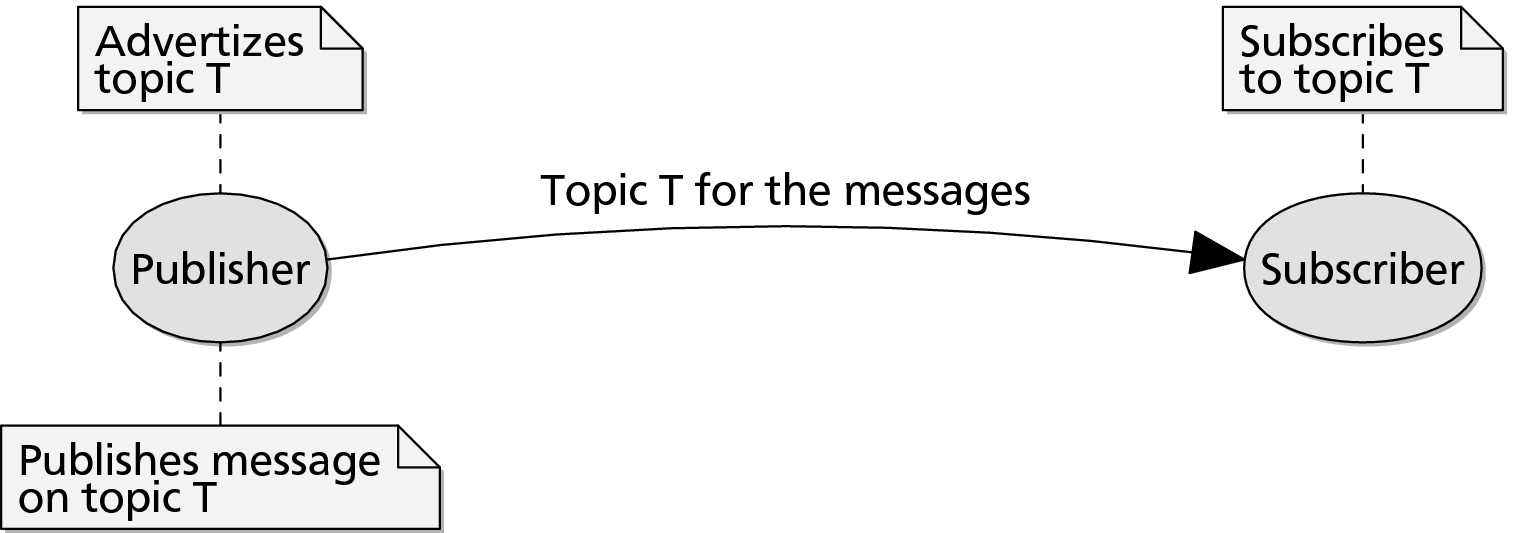
\includegraphics[width=1.0\textwidth]{ros-pub-sub}
		\caption{Modelo Publisher-Subscriber}
		\label{fig:ros-pub-sub}
	\end{figure}
	\chapter{Prueba con nodos ROS}
Asumiendo que ya tenemos creadas varios nodos de ROS conectados entre si, a los cuales denominaremos como \textbf{ros1}, \textbf{ros2} y \textbf{ros3}, vamos a crear un pequeño ejemplo de este tipo para comprender mejor su funcionamiento. En el ejemplo, El publisher publicará una serie de datos, que será recibidos por el subscriber una vez se haya suscrito al topic en el que se estén publicando. Para hacerlo lo más simple posible, los datos que se pasarán serán una serie de números enteros.

Nos basaremos en uno de los ejemplos de los que disponemos en la Wiki de ROS \cite{ros-tutorials}, al que haremos unos pequeños cambios para adaptarlo.

	\section{Código de la prueba}
	El código se divide en dos ficheros .cpp en los que tendremos por una parte el publisher y en la otra el subscriber.	Tendremos un tercer ahrivo más, que será el archivo CMakeLists.txt que nos servirá a la hora de construir el paquete.
	
		\subsection{Publisher}
		\lstinputlisting[style=cpp,numbers=left]{../code/pub-sub-example/talker.cpp}
		
		\subsection{Subscriber}
		\lstinputlisting[style=cpp,numbers=left]{../code/pub-sub-example/listener.cpp}
		
		\subsection{CMakeLists}
		\lstinputlisting[style=makefile,numbers=left]{../code/pub-sub-example/CMakeLists.txt}
	
	\section{Construir el paquete}
	Una vez programado el sistema, pasamos a compilarlo y construirlo. Basándonos en lo que se comentó en el capítulo anterior, lo haremos de la siguiente manera.
	
	\begin{lstlisting}[style=consola,numbers=left]
~$ mkdir -p ~/catkin_ws/src
~$ cd ~/catkin_ws/src
~/catkin_ws/src$ catkin_init_workspace
Creating symlink "/home/ander/catkin_ws/src/CMakeLists.txt" pointing to "/opt/ros/indigo/share/catkin/cmake/toplevel.cmake"
~/catkin_ws/src$ cd ..
~/catkin_ws$ source devel/setup.bash
bash: devel/setup.bash: No existe el archivo o el directorio
~/catkin_ws$ cd src/
~/catkin_ws/src$ catkin_create_pkg prueba std_msgs rospy roscpp
Created file prueba/package.xml
Created file prueba/CMakeLists.txt
Created folder prueba/include/prueba
Created folder prueba/src
Successfully created files in /home/ander/catkin_ws/src/prueba. Please adjust the values in package.xml.
~/catkin_ws/src$ ls
CMakeLists.txt  pruebaROS
~/catkin_ws/src$ cd ..
~/catkin_ws$ catkin_make
Base path: /home/ander/catkin_ws
Source space: /home/ander/catkin_ws/src
Build space: /home/ander/catkin_ws/build
Devel space: /home/ander/catkin_ws/devel
Install space: /home/ander/catkin_ws/install
####
#### Running command: "cmake /home/ander/catkin_ws/src -DCATKIN_DEVEL_PREFIX=/home/ander/catkin_ws/devel -DCMAKE_INSTALL_PREFIX=/home/ander/catkin_ws/install -G Unix Makefiles" in "/home/ander/catkin_ws/build"
####
-- The C compiler identification is GNU 4.8.4
-- The CXX compiler identification is GNU 4.8.4
-- Check for working C compiler: /usr/bin/cc
-- Check for working C compiler: /usr/bin/cc -- works
-- Detecting C compiler ABI info
-- Detecting C compiler ABI info - done
-- Check for working CXX compiler: /usr/bin/c++
-- Check for working CXX compiler: /usr/bin/c++ -- works
-- Detecting CXX compiler ABI info
-- Detecting CXX compiler ABI info - done
-- Using CATKIN_DEVEL_PREFIX: /home/ander/catkin_ws/devel
-- Using CMAKE_PREFIX_PATH: /opt/ros/indigo
-- This workspace overlays: /opt/ros/indigo
-- Found PythonInterp: /usr/bin/python (found version "2.7.6")
-- Using PYTHON_EXECUTABLE: /usr/bin/python
-- Using Debian Python package layout
-- Using empy: /usr/bin/empy
-- Using CATKIN_ENABLE_TESTING: ON
-- Call enable_testing()
-- Using CATKIN_TEST_RESULTS_DIR: /home/ander/catkin_ws/build/test_results
-- Looking for include file pthread.h
-- Looking for include file pthread.h - found
-- Looking for pthread_create
-- Looking for pthread_create - not found
-- Looking for pthread_create in pthreads
-- Looking for pthread_create in pthreads - not found
-- Looking for pthread_create in pthread
-- Looking for pthread_create in pthread - found
-- Found Threads: TRUE  
-- Found gtest sources under '/usr/src/gtest': gtests will be built
-- Using Python nosetests: /usr/bin/nosetests-2.7
-- catkin 0.6.14
-- BUILD_SHARED_LIBS is on
-- ~~~~~~~~~~~~~~~~~~~~~~~~~~~~~~~~~~~~~~~~~~~~~~~~~
-- ~~  traversing 1 packages in topological order:
-- ~~  - prueba
-- ~~~~~~~~~~~~~~~~~~~~~~~~~~~~~~~~~~~~~~~~~~~~~~~~~
-- +++ processing catkin package: 'pruebaROS'
-- ==> add_subdirectory(pruebaROS)
-- Configuring done
-- Generating done
-- Build files have been written to: /home/ander/catkin_ws/build
####
#### Running command: "make -j1 -l1" in "/home/ander/catkin_ws/build"
####
~/catkin_ws$ ls
build  devel  src
~/catkin_ws$ cd src
~/catkin_ws/src$ ls
CMakeLists.txt  prueba
~/catkin_ws/src$ cd prueba/
~/catkin_ws/src/prueba$ ls
CMakeLists.txt  include  package.xml  src
~/catkin_ws/src/prueba$ cd src
~/catkin_ws/src/prueba/src$ ls
~/catkin_ws/src/prueba/src$ touch talker.cpp
~/catkin_ws/src/prueba/src$ touch listener.cpp
~/catkin_ws/src/prueba/src$ ls
listener.cpp  talker.cpp

	\end{lstlisting}

	Ahora ya tenemos todos los archivos creados, debemos llenarlos con el contenido que hemos mostrado antes. En este caso uso \textit{nano} para editar los archivos, pero se puede hacer con \textit{vi} o cualquier otro editor.

	\begin{lstlisting}[style=consola,numbers=left]
~/catkin_ws/src/prueba/src$ nano listener.cpp
~/catkin_ws/src/prueba/src$ nano talker.cpp
~/catkin_ws/src/prueba/src$ cd ..
~/catkin_ws/src/prueba$ ls
CMakeLists.txt  include  package.xml  src
~/catkin_ws/src/prueba$ echo "" > CMakeLists.txt # Para vaciar el archivo
~/catkin_ws/src/prueba$ nano CMakeLists.txt
	\end{lstlisting}

	Una vez llenos podemos proceder a compilarlo.
	
	\begin{lstlisting}[style=consola,numbers=left]
~/catkin_ws/src/prueba$ cd ..
~/catkin_ws/src$ cd ..
~/catkin_ws$ ls
build  devel  src
~/catkin_ws$ catkin_make
ander@ubuntu-VirtualBox:~/catkin_ws$ catkin_make
Base path: /home/ander/catkin_ws
Source space: /home/ander/catkin_ws/src
Build space: /home/ander/catkin_ws/build
Devel space: /home/ander/catkin_ws/devel
Install space: /home/ander/catkin_ws/install
####
#### Running command: "cmake /home/ander/catkin_ws/src -DCATKIN_DEVEL_PREFIX=/home/ander/catkin_ws/devel -DCMAKE_INSTALL_PREFIX=/home/ander/catkin_ws/install -G Unix Makefiles" in "/home/ander/catkin_ws/build"
####
-- Using CATKIN_DEVEL_PREFIX: /home/ander/catkin_ws/devel
-- Using CMAKE_PREFIX_PATH: /home/ander/catkin_ws/devel;/opt/ros/indigo
-- This workspace overlays: /home/ander/catkin_ws/devel;/opt/ros/indigo
-- Using PYTHON_EXECUTABLE: /usr/bin/python
-- Using Debian Python package layout
-- Using empy: /usr/bin/empy
-- Using CATKIN_ENABLE_TESTING: ON
-- Call enable_testing()
-- Using CATKIN_TEST_RESULTS_DIR: /home/ander/catkin_ws/build/test_results
-- Found gtest sources under '/usr/src/gtest': gtests will be built
-- Using Python nosetests: /usr/bin/nosetests-2.7
-- catkin 0.6.14
-- BUILD_SHARED_LIBS is on
-- ~~~~~~~~~~~~~~~~~~~~~~~~~~~~~~~~~~~~~~~~~~~~~~~~~
-- ~~  traversing 1 packages in topological order:
-- ~~  - prueba
-- ~~~~~~~~~~~~~~~~~~~~~~~~~~~~~~~~~~~~~~~~~~~~~~~~~
-- +++ processing catkin package: 'prueba'
-- ==> add_subdirectory(prueba)
-- Configuring done
-- Generating done
-- Build files have been written to: /home/ander/catkin_ws/build
####
#### Running command: "make -j1 -l1" in "/home/ander/catkin_ws/build"
####
Scanning dependencies of target listener
[ 50%] Building CXX object prueba/CMakeFiles/listener.dir/src/listener.cpp.o
Linking CXX executable /home/ander/catkin_ws/devel/lib/prueba/listener
[ 50%] Built target listener
Scanning dependencies of target talker
[100%] Building CXX object prueba/CMakeFiles/talker.dir/src/talker.cpp.o
Linking CXX executable /home/ander/catkin_ws/devel/lib/prueba/talker
[100%] Built target talker
	\end{lstlisting}
	
	Esto nos generará dos ejecutables, \emph{talker} y \emph{listener}, que por defecto irán al directorio devel/lib/[nombre del paquete] de nuestro workspace.
	
	\begin{lstlisting}[style=consola,numbers=left]

	\end{lstlisting}
	
	\section{Ejecución}
	Probaremos el sistema para comprobar que funciona correctamente. Para ello haremos lo siguiente.
	
	\begin{lstlisting}[style=consola,numbers=left]
	
	\end{lstlisting}
	
\part{Implementación del sistema}
	\chapter{Creación del sistema}

El sistema que vamos a crear constará de las siguientes partes. Primero sobre las máquinas con SO Windows se instalará una máquina virtual Ubuntu sobre Virtualbox para trabajar en un entorno linux. A día de hoy existen formas de trabajar directamente con Docker en sistemas Windows tanto por CLI (Command Line Interface) como a través de una interfaz gráfica, aunque éstas se basan en emular el kernel de linux. Para este caso se ha optado por trabajar en un entorno linux conocido para hacer más simple el despligue del sistema.

Dentro de dicha máquina Ubuntu se instalará el propio Docker. Mediante Docker crearemos diferentes contenedores. Cada uno de esos contenedores se crearán a partir de una imagen de Ubuntu que vendrá con ROS instalado. Esa imagen sera la que aparece en el Docker Hub como \emph{osrf/ros:indigo-desktop}. Estas máquinas se comunicarán entre ellas mediante una red creada con la herramienta \emph{network} de Docker.

El esquema del sistema vendría a ser el que se muestra en la Figura \ref{fig:esquemaOriginal}.
\begin{figure}[H] % Con el parámetro H la imagens se muestra justo en el sitio en el que se ha definido
	\centering
	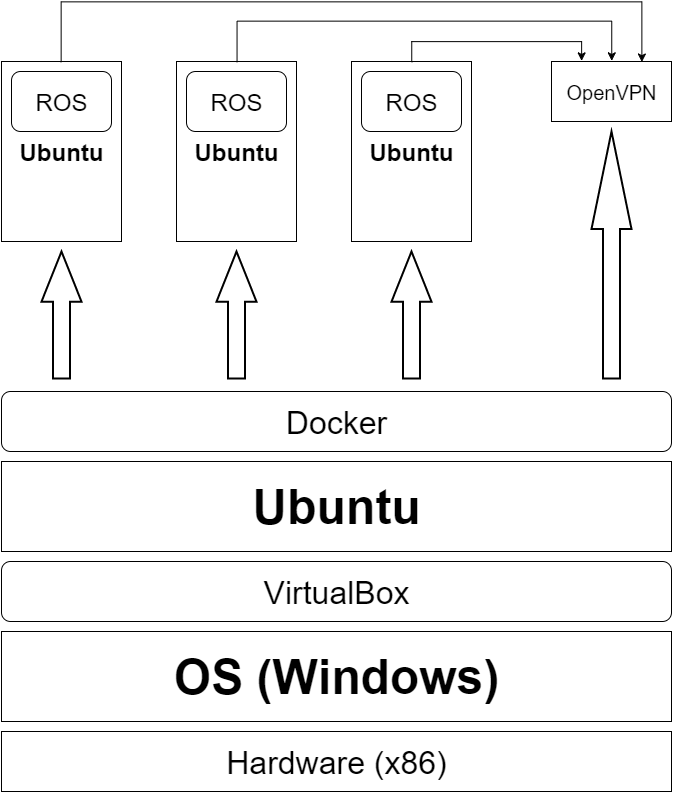
\includegraphics[width=0.8\textwidth]{esquemaOriginal}
	%		\includesvg{figuras/esquemaOriginal}
	\caption{Esquema del sistema en un ordenador x86}
	\label{fig:esquemaOriginal}
\end{figure}

Posteriormente integraremos nuestro sistema en una Raspberry Pi. El esquema del sistema aplicado en una Raspberry Pi se muestra en la Figura \ref{fig:esquemaRPi}.
\begin{figure}[H]
	\centering
	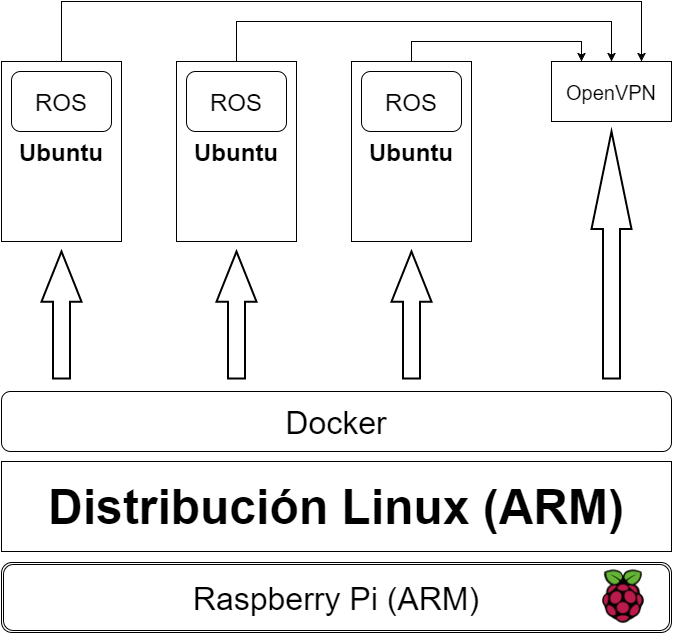
\includegraphics[width=0.8\textwidth]{esquemaRPi}
	%		\includesvg{figuras/esquemaRPi}
	\caption{Esquema del sistema en una Raspberry Pi}
	\label{fig:esquemaRPi}
\end{figure}

	\section{Crear el sistema con Docker}
	Lo primero que haremos será crear una serie de contenedores de docker con ROS dentro.
	
	\begin{enumerate}
		\item Creamos en tres terminales diferentes tres contenedores ROS.
		\begin{lstlisting}[style=consola,numbers=left]
$ docker run --name ros0 -it osrf/ros:indigo-desktop
$ docker run --name ros1 -it osrf/ros:indigo-desktop
$ docker run --name ros2 -it osrf/ros:indigo-desktop
		\end{lstlisting}
		
		\item Desde el host, creamos la red y conectamos los tres contenedores a ella.
		\begin{lstlisting}[style=consola,numbers=left]
$ docker network create red
a9ccfbd91df31be74881c7a7e65fbb0fdd6fec286debec6c72b1f627bb0e2ad0
$ docker network ls
NETWORK ID          NAME                DRIVER
a9ccfbd91df3        red                 bridge              
6fb4fab5cc04        bridge              bridge              
a55fc7d11d74        none                null                
2c96fadb05a4        host                host                
$ docker network connect red ros0
$ docker network connect red ros1
$ docker network connect red ros2
		\end{lstlisting}
		
		\item Probamos el ejemplo anterior con nodos ROS pero esta vez dentro de los contenedores Docker. Simplemente hay que tener en cuenta que hay que configurar la variable \emph{ROS\_MASTER\_URI} para que apunte a \emph{ros0}, que es la dirección del contenedor que ejecutará \emph{roscore}.
		
		\begin{enumerate}
			\item Lanzamos \emph{roscore} en \emph{ros0}.
			\begin{lstlisting}[style=consola]
root@d55b47478e2c:/# roscore
			\end{lstlisting}
			
			\item En \emph{ros1} y \emph{ros2} configuramos la variable que indica donde se está ejecutando \emph{roscore}
			\begin{lstlisting}[style=consola]
$ ROS_MASTER_URI=http://ros0:11311/
			\end{lstlisting}
			
			\item Tanto para \emph{ros1} como para \emph{ros2}, hace falta poner en la variable \emph{ROS\_IP} la IP del conentedor. Esto sirve para que el \emph{roscore} pueda encontrar los nodos. Lo haremos mirando dentro de cada contenedor la IP \textbf{correspondiente a la red creada por nosotros}. En nuestro caso se haría de la siguiente manera.
			\begin{lstlisting}[style=consola]
root@9d1dbcbf599c:~/catkin_ws# export ROS_IP=172.18.0.4
root@ee37147629e4:~/catkin_ws# export ROS_IP=172.18.0.3
			\end{lstlisting}
			
			\item Con todo el ejemplo creado y compilado dentro de \emph{ros1} y \emph{ros2}, lanzamos en \emph{ros1} el listener.
			\begin{lstlisting}[style=consola]
root@9d1dbcbf599c:~/# rosrun prueba listener	
			\end{lstlisting}
			
			\item Y probamos a escribir mediante el talker.
			\begin{lstlisting}[style=consola]
root@9d1dbcbf599c:~/# rostopic pub -1 /chatter std_msgs/String PruebaMensaje
			\end{lstlisting}
			\begin{lstlisting}[style=consola]
root@9d1dbcbf599c:~/# rosrun prueba listener
[ INFO] [1447688515.499505438]: I heard: [PruebaMensaje]
			\end{lstlisting}

		\end{enumerate}
		
	\end{enumerate}
	
	\section{Aplicaciones para el sistema}
		{\color{red} ...en desarrollo}

%----------------------------------------------------------------------------------------

\backmatter

% Bibliografía, glosario, ...
\bibliographystyle{plainnat}
\bibliography{biblio}

\end{document}
%========================================================================================